\documentclass{article}[12pt]
\setlength{\parskip}{\baselineskip}
\setlength{\parindent}{0pt}

\renewcommand{\baselinestretch}{1.5}

\usepackage[affil-it]{authblk}
\usepackage[space]{grffile}

\usepackage[a4paper]{geometry}
\geometry{verbose}

\usepackage{float}
\usepackage{graphicx}
\graphicspath{{figures/}}

\usepackage{setspace}
\usepackage{caption}

\usepackage[utf8]{inputenc}
\usepackage[english]{babel}

\usepackage{latexsym,textcomp,longtable,tabulary}
\usepackage{booktabs,array,multirow,braket}
\usepackage{amsfonts,amsmath,amssymb,mathbbol,calc}
\usepackage{subfigure,color,blindtext,enumitem,siunitx}
\usepackage[colorinlistoftodos]{todonotes}

\usepackage{mathtools}
\usepackage{url,hyperref,etoolbox}
\numberwithin{equation}{section}
\hypersetup{colorlinks=false,pdfborder={0 0 0}}

%+figure layout options
\restylefloat{figure}
\setlist{leftmargin=*,before=\setlength{\rightmargin}{\leftmargin}}
%-figure layout options

\providecommand\citet{\cite}
\providecommand\citep{\cite}
\providecommand\citealt{\cite}

\makeatletter
\makeatother

\begin{document}

\title{
Time-series segmentation and latent\\ representation of musical instruments
}

\author{Gregory Szep}
\affil{King's College London}
\date{\today}
\maketitle
\vspace{-3em}
\abstract{
\noindent
Music information retrieval tasks serve as faithful benchmarks for
time-series analysis pipelines due to the availability of strongly labelled
training data such as MusicNet. Clustering algorithms in spectral sub-spaces,
hidden Markov models and causal convolutional neural networks are compared in
their ability to transform time-series to a continuous latent space that
clusters eleven orchestral instruments. The latent space is evaluated
quantitatively with precision-recall metrics obtained by comparing the
instrument prediction from a segment of audio to the ground truth obtained
from musical scores, and qualitatively by generating samples of audio for given
regions in the latent space.}

\section{Methodology Outline}
\subsection{Mapping time-series to latent space}
The input data are single channel time-series points $\mathcal{D}=\{x(t_1)\dots
x(t_N)\}$ sampled at frequency $f$ from an underlying continuous state-time
process $x(t)$, that is the oscillating sound waves emitted by a live orchestra.
\\\\
For each time point there is a musical score $\bar{\mathrm{L}}(t)\in[0,128]^L$ which
represents the midi notes played by $L$ instruments of a particular note on a particular instrument. These scores
are composed by $Y$ instrument activations $\bar{\mathrm{y}}(t)\in[0,1]^Y$ and $N$
note activations $\bar{\mathrm{n}}(t)\in[0,1]^N$.
\\\\
The task is to recover instrument activations $\bar{\mathrm{y}}(t)$ from
the input signal $x(t)$. Within unsupervised methods this task is known as
under-determined blind source separation. When the number of input channels
equals to the number of sources this problem is fully determined and can be
solved using independent component analysis
\cite{Platt1995Information-MaximizationDeconvolution} and other algorithms
that search for sparse representations. Through the lens of supervised approaches
this problem can be seen as an audio segmentation task. In recent years
convolutional networks have demonstrated success in image segmentation \cite{},
whos architectures are adaptable to audio data.
\\\\
The principal assumption in this task is that $x(t)$ is a linear superposition
of sources and that in some latent space $\bar{\mathrm{z}}(t)$ these sources are
linearly separable. The optimal latent space mapping $f$ should minimise the
cost function $J[f]$, which in general is some norm $\left\lVert\,\right\rVert$
of the error subject to some complexity measure $S[f]$. The data in the latent
space should be separable by a suitable choice of unmixing matrix $\mathbf{W}$.
\begin{align}
	J[f]=\left\lVert\bar{\mathrm{y}}(t)-\mathbf{W}\,\bar{\mathrm{z}}(t)\right\rVert+S[f]
	\quad\text{where}\quad
	\bar{\mathrm{z}}(t) = f(x,t)\\
	\exists\,\mathbf{W},f\,:\,f=\underset{f'}{\mathrm{argmin}}\,J[f']
	\qquad\qquad\qquad
\end{align}
Note that the map $f$ is most likely not one-to-one respect to $t$. It is not a
single time point but a time window that encodes which instrument is being
played. While linear separability via $\mathbf{W}$ by is sufficient it is not
necessary; one could instead simply look for clusters.

\subsubsection{Wavelet transforms and independent components}
The naive approach would be to attempt to guess the mapping $f$ via suitable
phenomenological agruments. It is reasonable to suppose that one could separate
instruments based on their spectral signature at any moment in time. The decibel
spectrogram $S(\omega,t)$ is obtained by taking the $\log_{10}$ absolute value
of a short-time fourier transform.
\begin{align}
	S(\omega,t):=\log_{10}\left[\left|\,
	\int_{-\infty}^{\infty}\!
		x(\tau)\mathbb{e}^{-\mathbb{i}\omega \tau}h(\tau-t)
	\,\mathrm{d}\tau
	\,\right|\right]
\end{align}
A suitable window function $h(t)$ must be chosen; different choices lead to
different amounts of spectral leakage and time-frequency domain resolution
\cite{}. For demonstration purposes a ~46ms wide Hann window is chosen with a
stride of ~3ms, which is on the order of the shortest duration of a musical
sound.

\begin{figure}[H]
\centering{}
\captionsetup{justification=centering}
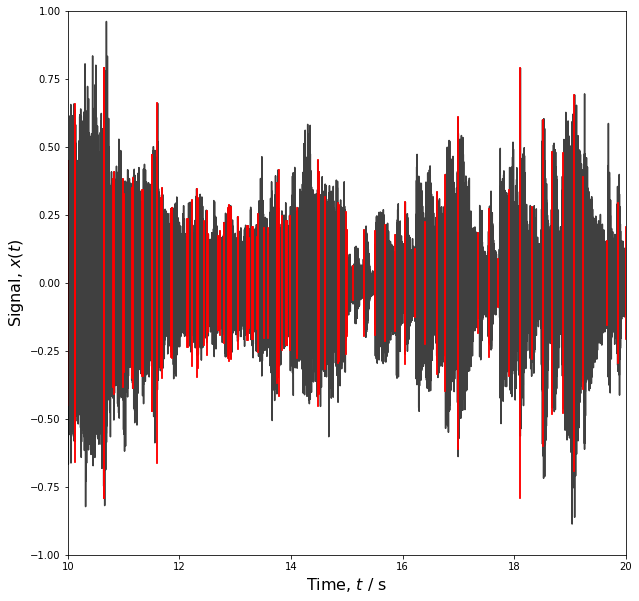
\includegraphics[scale=0.5]{signal}
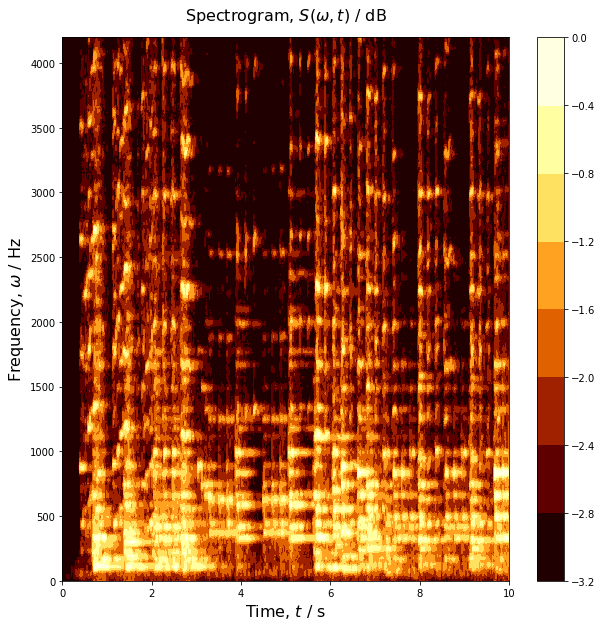
\includegraphics[scale=0.5]{spectrogram}
\caption{
Raw input signal (top) labelled by instrument activation $\bar{\mathrm{y}}(t)$
and its corresponding spectrogram (bottom)
}
\label{fig:methods}
\end{figure}

The spectral signature of the input signal at a given time $t$ can be
represented as a point in $F$ dimensional point, where $F$ is the number
of frequency bins up to a given cutoff frequency. $F=500$
\begin{enumerate}
	\item get spectrogram using windowed Fourier transform or Gabor transforms,
	discuss spectral leakage, contrast, normalisation and noise filtering in an
	unsupervised way
	\item perform principal components and independent component dimensionality
	reduction along frequency dimension, discuss differences between them.
\end{enumerate}
\subsubsection{Markov models and expectation-maximisation}
\begin{enumerate}
	\item discuss implementations of random Markov fields in image segmentation
	and how they can be adapted to audio segmentation
	\item random Markov field vs hidden Markov model?
	\item expectation-maximisation vs error back-propagation
\end{enumerate}
\subsubsection{Feature extraction with causal convolutions}
Convolutional architectures have become popular due to their ability to compress spatio-temporal
information for discrimination and generation tasks \cite{Oord2016a,Goodfellow}.
A causal convolutional network \cite{Oord2016} --- which encodes the arrow of time in
its architecture --- is trained for the audio segmentation task.
\begin{enumerate}
	\item dilated causal convolutions as a merge between a feature
	extractor and a dimensionality reduction technique. This is a supervised method
	\item Compare clusters to those obtained in Section 1.1.1
\end{enumerate}
\subsection{Clustering in latent space}
\begin{enumerate}
	\item We have a hierarchical clustering problem: there are 11 instruments each
	of which can play 28-83 notes. The easier problem is to only cluster instruments,
	the harder problem is to cluster both instruments and notes.
\end{enumerate}

\subsubsection{K-means}

\begin{enumerate}
	\item Since we know how many instruments there are, we can apply a naive K-means
	and see what happens. Here the disadvantage is that time-ordering may be
	ignored, which can lead to noisy/discontinuous audio segment classifications
	\item Discuss de-noising strategies in post-classification: possibly Markov
	random fields from section 1.1.2?
\end{enumerate}

\subsubsection{Fully convolutional networks}
\begin{enumerate}
	\item I shall attempt to adapt the the fully convolutional architecture \cite{Long2015}
	for the audio segmentation task. Discuss advantages of end-to-end trained solution.
\end{enumerate}

\subsection{Evaluation methods}
\subsubsection{Audio segment retrieval}
\begin{enumerate}
	\item outline of object detection / segmentation in image analysis
	\item precision-recall metric applied to audio
\end{enumerate}
\subsubsection{Instrument generation}
\begin{enumerate}
	\item introduction to encoder / decoder pipelines as generative models which
	can produce data given activation of input in latent space.
	\item attempt to produce sounds that are interpolations between
	existing instruments, assess qualitatively how realistic they sound
\end{enumerate}


\begin{figure}[H]
\centering{}
\captionsetup{justification=centering}
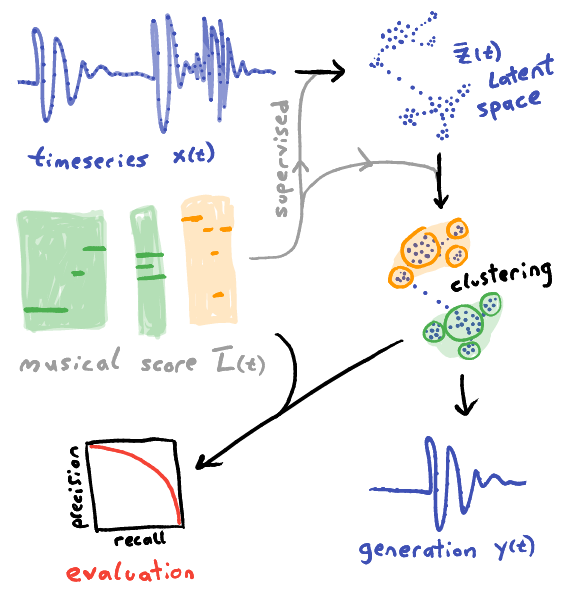
\includegraphics[scale=0.5]{methods}
\caption{Summary of methodology showing all stages of the audio segmentation task.\\
Each transition between sub-figures can be achieved with appropriate algorithms
}
\label{fig:methods}
\end{figure}

\section{Dataset Description}

\subsection{Input and Labels}
\begin{enumerate}
	\item small summary table of the MusicNet dataset \cite{Thickstun2016}, advantages
	over EEG and other bio-sensory data for bench-marking signal processing algorithms
	\item raw labels are time aligned transcripts of the sheet music. How to we
	parse that into instrument activations and note activations.
	\item cross-validation --- if any
\end{enumerate}

\subsection{Data Partitioning}
\begin{enumerate}
	\item test, validation and train sets
	\item cross-validation --- if any
\end{enumerate}

\section{Results, Protocols and Conclusions}
\begin{enumerate}
	\item all relevant figures will be presented here
\end{enumerate}
\subsection{Learned feature maps}

\subsection{Clustering performance}

\subsection{Generating instruments}

\bibliography{mendeley_v2}
\bibliographystyle{ieeetr}
\end{document}
